%% bare_jrnl_compsoc.tex
%% V1.3
%% 2007/01/11
%% by Michael Shell
%% See:
%% http://www.michaelshell.org/
%% for current contact information.
%%
%% This is a skeleton file demonstrating the use of IEEEtran.cls
%% (requires IEEEtran.cls version 1.7 or later) with an IEEE Computer
%% Society journal paper.
%%
%% Support sites:
%% http://www.michaelshell.org/tex/ieeetran/
%% http://www.ctan.org/tex-archive/macros/latex/contrib/IEEEtran/
%% and
%% http://www.ieee.org/

%%*************************************************************************
%% Legal Notice:
%% This code is offered as-is without any warranty either expressed or
%% implied; without even the implied warranty of MERCHANTABILITY or
%% FITNESS FOR A PARTICULAR PURPOSE! 
%% User assumes all risk.
%% In no event shall IEEE or any contributor to this code be liable for
%% any damages or losses, including, but not limited to, incidental,
%% consequential, or any other damages, resulting from the use or misuse
%% of any information contained here.
%%
%% All comments are the opinions of their respective authors and are not
%% necessarily endorsed by the IEEE.
%%
%% This work is distributed under the LaTeX Project Public License (LPPL)
%% ( http://www.latex-project.org/ ) version 1.3, and may be freely used,
%% distributed and modified. A copy of the LPPL, version 1.3, is included
%% in the base LaTeX documentation of all distributions of LaTeX released
%% 2003/12/01 or later.
%% Retain all contribution notices and credits.
%% ** Modified files should be clearly indicated as such, including  **
%% ** renaming them and changing author support contact information. **
%%
%% File list of work: IEEEtran.cls, IEEEtran_HOWTO.pdf, bare_adv.tex,
%%                    bare_conf.tex, bare_jrnl.tex, bare_jrnl_compsoc.tex
%%*************************************************************************

% *** Authors should verify (and, if needed, correct) their LaTeX system  ***
% *** with the testflow diagnostic prior to trusting their LaTeX platform ***
% *** with production work. IEEE's font choices can trigger bugs that do  ***
% *** not appear when using other class files.                            ***
% The testflow support page is at:
% http://www.michaelshell.org/tex/testflow/




% Note that the a4paper option is mainly intended so that authors in
% countries using A4 can easily print to A4 and see how their papers will
% look in print - the typesetting of the document will not typically be
% affected with changes in paper size (but the bottom and side margins will).
% Use the testflow package mentioned above to verify correct handling of
% both paper sizes by the user's LaTeX system.
%
% Also note that the "draftcls" or "draftclsnofoot", not "draft", option
% should be used if it is desired that the figures are to be displayed in
% draft mode.
%
% The Computer Society usually requires 12pt for submissions.
%
\documentclass[10pt,journal,compsoc]{IEEEtran}
%
% If IEEEtran.cls has not been installed into the LaTeX system files,
% manually specify the path to it like:
% \documentclass[12pt,journal,compsoc]{../sty/IEEEtran}


\usepackage[utf8]{inputenc}
\usepackage[T1]{fontenc}
\usepackage{listings}

\newcommand{\reffig}[1]{Fig. \ref{#1}}
%% \usepackage{lmodern} % vector font, ikke bitmap!!
%% \usepackage{wrapfig}
%% \usepackage{verbatim}
%% \usepackage{subfig}
%% \usepackage{slashbox}

% Some very useful LaTeX packages include:
% (uncomment the ones you want to load)


% *** MISC UTILITY PACKAGES ***
%
%\usepackage{ifpdf}
% Heiko Oberdiek's ifpdf.sty is very useful if you need conditional
% compilation based on whether the output is pdf or dvi.
% usage:
% \ifpdf
%   % pdf code
% \else
%   % dvi code
% \fi
% The latest version of ifpdf.sty can be obtained from:
% http://www.ctan.org/tex-archive/macros/latex/contrib/oberdiek/
% Also, note that IEEEtran.cls V1.7 and later provides a builtin
% \ifCLASSINFOpdf conditional that works the same way.
% When switching from latex to pdflatex and vice-versa, the compiler may
% have to be run twice to clear warning/error messages.






% *** CITATION PACKAGES ***
%
\ifCLASSOPTIONcompsoc
  % IEEE Computer Society needs nocompress option
  % requires cite.sty v4.0 or later (November 2003)
  \usepackage[nocompress]{cite}
\else
  % normal IEEE
  \usepackage{cite}
\fi
\usepackage[plainpages=false]{hyperref}
% cite.sty was written by Donald Arseneau
% V1.6 and later of IEEEtran pre-defines the format of the cite.sty package
% \cite{} output to follow that of IEEE. Loading the cite package will
% result in citation numbers being automatically sorted and properly
% "compressed/ranged". e.g., [1], [9], [2], [7], [5], [6] without using
% cite.sty will become [1], [2], [5]--[7], [9] using cite.sty. cite.sty's
% \cite will automatically add leading space, if needed. Use cite.sty's
% noadjust option (cite.sty V3.8 and later) if you want to turn this off.
% cite.sty is already installed on most LaTeX systems. Be sure and use
% version 4.0 (2003-05-27) and later if using hyperref.sty. cite.sty does
% not currently provide for hyperlinked citations.
% The latest version can be obtained at:
% http://www.ctan.org/tex-archive/macros/latex/contrib/cite/
% The documentation is contained in the cite.sty file itself.
%
% Note that some packages require special options to format as the Computer
% Society requires. In particular, Computer Society  papers do not use
% compressed citation ranges as is done in typical IEEE papers
% (e.g., [1]-[4]). Instead, they list every citation separately in order
% (e.g., [1], [2], [3], [4]). To get the latter we need to load the cite
% package with the nocompress option which is supported by cite.sty v4.0
% and later. Note also the use of a CLASSOPTION conditional provided by
% IEEEtran.cls V1.7 and later.





% *** GRAPHICS RELATED PACKAGES ***
%
\ifCLASSINFOpdf
  \usepackage[pdftex]{graphicx}
  % declare the path(s) where your graphic files are
  \graphicspath{{pics/}}
  % and their extensions so you won't have to specify these with
  % every instance of \includegraphics
  \DeclareGraphicsExtensions{.pdf,.jpeg,.png}
\else
  % or other class option (dvipsone, dvipdf, if not using dvips). graphicx
  % will default to the driver specified in the system graphics.cfg if no
  % driver is specified.
  % \usepackage[dvips]{graphicx}
  % declare the path(s) where your graphic files are
  % \graphicspath{{../eps/}}
  % and their extensions so you won't have to specify these with
  % every instance of \includegraphics
  % \DeclareGraphicsExtensions{.eps}
\fi
% graphicx was written by David Carlisle and Sebastian Rahtz. It is
% required if you want graphics, photos, etc. graphicx.sty is already
% installed on most LaTeX systems. The latest version and documentation can
% be obtained at: 
% http://www.ctan.org/tex-archive/macros/latex/required/graphics/
% Another good source of documentation is "Using Imported Graphics in
% LaTeX2e" by Keith Reckdahl which can be found as epslatex.ps or
% epslatex.pdf at: http://www.ctan.org/tex-archive/info/
%
% latex, and pdflatex in dvi mode, support graphics in encapsulated
% postscript (.eps) format. pdflatex in pdf mode supports graphics
% in .pdf, .jpeg, .png and .mps (metapost) formats. Users should ensure
% that all non-photo figures use a vector format (.eps, .pdf, .mps) and
% not a bitmapped formats (.jpeg, .png). IEEE frowns on bitmapped formats
% which can result in "jaggedy"/blurry rendering of lines and letters as
% well as large increases in file sizes.
%
% You can find documentation about the pdfTeX application at:
% http://www.tug.org/applications/pdftex





% *** MATH PACKAGES ***
%
\usepackage[cmex10]{amsmath}
% A popular package from the American Mathematical Society that provides
% many useful and powerful commands for dealing with mathematics. If using
% it, be sure to load this package with the cmex10 option to ensure that
% only type 1 fonts will utilized at all point sizes. Without this option,
% it is possible that some math symbols, particularly those within
% footnotes, will be rendered in bitmap form which will result in a
% document that can not be IEEE Xplore compliant!
%
% Also, note that the amsmath package sets \interdisplaylinepenalty to 10000
% thus preventing page breaks from occurring within multiline equations. Use:
%\interdisplaylinepenalty=2500
% after loading amsmath to restore such page breaks as IEEEtran.cls normally
% does. amsmath.sty is already installed on most LaTeX systems. The latest
% version and documentation can be obtained at:
% http://www.ctan.org/tex-archive/macros/latex/required/amslatex/math/





% *** SPECIALIZED LIST PACKAGES ***
%
%\usepackage{algorithmic}
% algorithmic.sty was written by Peter Williams and Rogerio Brito.
% This package provides an algorithmic environment fo describing algorithms.
% You can use the algorithmic environment in-text or within a figure
% environment to provide for a floating algorithm. Do NOT use the algorithm
% floating environment provided by algorithm.sty (by the same authors) or
% algorithm2e.sty (by Christophe Fiorio) as IEEE does not use dedicated
% algorithm float types and packages that provide these will not provide
% correct IEEE style captions. The latest version and documentation of
% algorithmic.sty can be obtained at:
% http://www.ctan.org/tex-archive/macros/latex/contrib/algorithms/
% There is also a support site at:
% http://algorithms.berlios.de/index.html
% Also of interest may be the (relatively newer and more customizable)
% algorithmicx.sty package by Szasz Janos:
% http://www.ctan.org/tex-archive/macros/latex/contrib/algorithmicx/




% *** ALIGNMENT PACKAGES ***
%
%\usepackage{array}
% Frank Mittelbach's and David Carlisle's array.sty patches and improves
% the standard LaTeX2e array and tabular environments to provide better
% appearance and additional user controls. As the default LaTeX2e table
% generation code is lacking to the point of almost being broken with
% respect to the quality of the end results, all users are strongly
% advised to use an enhanced (at the very least that provided by array.sty)
% set of table tools. array.sty is already installed on most systems. The
% latest version and documentation can be obtained at:
% http://www.ctan.org/tex-archive/macros/latex/required/tools/


%\usepackage{mdwmath}
%\usepackage{mdwtab}
% Also highly recommended is Mark Wooding's extremely powerful MDW tools,
% especially mdwmath.sty and mdwtab.sty which are used to format equations
% and tables, respectively. The MDWtools set is already installed on most
% LaTeX systems. The lastest version and documentation is available at:
% http://www.ctan.org/tex-archive/macros/latex/contrib/mdwtools/


% IEEEtran contains the IEEEeqnarray family of commands that can be used to
% generate multiline equations as well as matrices, tables, etc., of high
% quality.


%\usepackage{eqparbox}
% Also of notable interest is Scott Pakin's eqparbox package for creating
% (automatically sized) equal width boxes - aka "natural width parboxes".
% Available at:
% http://www.ctan.org/tex-archive/macros/latex/contrib/eqparbox/





% *** SUBFIGURE PACKAGES ***
\ifCLASSOPTIONcompsoc
\usepackage[tight,normalsize,sf,SF]{subfigure}
\else
\usepackage[tight,footnotesize]{subfigure}
\fi
% subfigure.sty was written by Steven Douglas Cochran. This package makes it
% easy to put subfigures in your figures. e.g., "Figure 1a and 1b". For IEEE
% work, it is a good idea to load it with the tight package option to reduce
% the amount of white space around the subfigures. Computer Society papers
% use a larger font and \sffamily font for their captions, hence the
% additional options needed under compsoc mode. subfigure.sty is already
% installed on most LaTeX systems. The latest version and documentation can
% be obtained at:
% http://www.ctan.org/tex-archive/obsolete/macros/latex/contrib/subfigure/
% subfigure.sty has been superceeded by subfig.sty.


%\ifCLASSOPTIONcompsoc
%  \usepackage[caption=false]{caption}
%  \usepackage[font=normalsize,labelfont=sf,textfont=sf]{subfig}
%\else
%  \usepackage[caption=false]{caption}
%  \usepackage[font=footnotesize]{subfig}
%\fi
% subfig.sty, also written by Steven Douglas Cochran, is the modern
% replacement for subfigure.sty. However, subfig.sty requires and
% automatically loads Axel Sommerfeldt's caption.sty which will override
% IEEEtran.cls handling of captions and this will result in nonIEEE style
% figure/table captions. To prevent this problem, be sure and preload
% caption.sty with its "caption=false" package option. This is will preserve
% IEEEtran.cls handing of captions. Version 1.3 (2005/06/28) and later 
% (recommended due to many improvements over 1.2) of subfig.sty supports
% the caption=false option directly:
%\ifCLASSOPTIONcompsoc
%  \usepackage[caption=false,font=normalsize,labelfont=sf,textfont=sf]{subfig}
%\else
%  \usepackage[caption=false,font=footnotesize]{subfig}
%\fi
%
% The latest version and documentation can be obtained at:
% http://www.ctan.org/tex-archive/macros/latex/contrib/subfig/
% The latest version and documentation of caption.sty can be obtained at:
% http://www.ctan.org/tex-archive/macros/latex/contrib/caption/




% *** FLOAT PACKAGES ***
%
%\usepackage{fixltx2e}
% fixltx2e, the successor to the earlier fix2col.sty, was written by
% Frank Mittelbach and David Carlisle. This package corrects a few problems
% in the LaTeX2e kernel, the most notable of which is that in current
% LaTeX2e releases, the ordering of single and double column floats is not
% guaranteed to be preserved. Thus, an unpatched LaTeX2e can allow a
% single column figure to be placed prior to an earlier double column
% figure. The latest version and documentation can be found at:
% http://www.ctan.org/tex-archive/macros/latex/base/



%\usepackage{stfloats}
% stfloats.sty was written by Sigitas Tolusis. This package gives LaTeX2e
% the ability to do double column floats at the bottom of the page as well
% as the top. (e.g., "\begin{figure*}[!b]" is not normally possible in
% LaTeX2e). It also provides a command:
%\fnbelowfloat
% to enable the placement of footnotes below bottom floats (the standard
% LaTeX2e kernel puts them above bottom floats). This is an invasive package
% which rewrites many portions of the LaTeX2e float routines. It may not work
% with other packages that modify the LaTeX2e float routines. The latest
% version and documentation can be obtained at:
% http://www.ctan.org/tex-archive/macros/latex/contrib/sttools/
% Documentation is contained in the stfloats.sty comments as well as in the
% presfull.pdf file. Do not use the stfloats baselinefloat ability as IEEE
% does not allow \baselineskip to stretch. Authors submitting work to the
% IEEE should note that IEEE rarely uses double column equations and
% that authors should try to avoid such use. Do not be tempted to use the
% cuted.sty or midfloat.sty packages (also by Sigitas Tolusis) as IEEE does
% not format its papers in such ways.




%\ifCLASSOPTIONcaptionsoff
%  \usepackage[nomarkers]{endfloat}
% \let\MYoriglatexcaption\caption
% \renewcommand{\caption}[2][\relax]{\MYoriglatexcaption[#2]{#2}}
%\fi
% endfloat.sty was written by James Darrell McCauley and Jeff Goldberg.
% This package may be useful when used in conjunction with IEEEtran.cls'
% captionsoff option. Some IEEE journals/societies require that submissions
% have lists of figures/tables at the end of the paper and that
% figures/tables without any captions are placed on a page by themselves at
% the end of the document. If needed, the draftcls IEEEtran class option or
% \CLASSINPUTbaselinestretch interface can be used to increase the line
% spacing as well. Be sure and use the nomarkers option of endfloat to
% prevent endfloat from "marking" where the figures would have been placed
% in the text. The two hack lines of code above are a slight modification of
% that suggested by in the endfloat docs (section 8.3.1) to ensure that
% the full captions always appear in the list of figures/tables - even if
% the user used the short optional argument of \caption[]{}.
% IEEE papers do not typically make use of \caption[]'s optional argument,
% so this should not be an issue. A similar trick can be used to disable
% captions of packages such as subfig.sty that lack options to turn off
% the subcaptions:
% For subfig.sty:
% \let\MYorigsubfloat\subfloat
% \renewcommand{\subfloat}[2][\relax]{\MYorigsubfloat[]{#2}}
% For subfigure.sty:
% \let\MYorigsubfigure\subfigure
% \renewcommand{\subfigure}[2][\relax]{\MYorigsubfigure[]{#2}}
% However, the above trick will not work if both optional arguments of
% the \subfloat/subfig command are used. Furthermore, there needs to be a
% description of each subfigure *somewhere* and endfloat does not add
% subfigure captions to its list of figures. Thus, the best approach is to
% avoid the use of subfigure captions (many IEEE journals avoid them anyway)
% and instead reference/explain all the subfigures within the main caption.
% The latest version of endfloat.sty and its documentation can obtained at:
% http://www.ctan.org/tex-archive/macros/latex/contrib/endfloat/
%
% The IEEEtran \ifCLASSOPTIONcaptionsoff conditional can also be used
% later in the document, say, to conditionally put the References on a 
% page by themselves.




% *** PDF, URL AND HYPERLINK PACKAGES ***
%
%\usepackage{url}
% url.sty was written by Donald Arseneau. It provides better support for
% handling and breaking URLs. url.sty is already installed on most LaTeX
% systems. The latest version can be obtained at:
% http://www.ctan.org/tex-archive/macros/latex/contrib/misc/
% Read the url.sty source comments for usage information. Basically,
% \url{my_url_here}.


% correct bad hyphenation here
\hyphenation{op-tical net-works semi-conduc-tor be-hand-linger aflejrings-kernel aflejrings-kernelen}


\begin{document}
%
% paper title
% can use linebreaks \\ within to get better formatting as desired
\title{Radiotherapy: Superposition/convolution implemented using fast raytracing}

%% \begin{figure}
%% \centering
%%   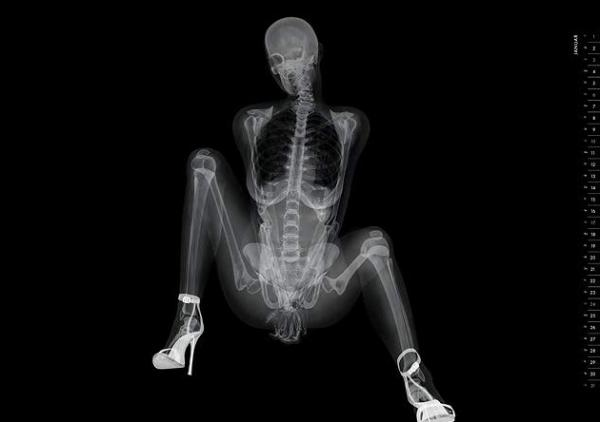
\includegraphics[width=8cm]{frontpage2}
%% \end{figure}

%
%
% Author names and IEEE memberships
% note positions of commas and nonbreaking spaces ( ~ ) LaTeX will not break
% a structure at a ~ so this keeps an author's name from being broken across
% two lines.
% use \thanks{} to gain access to the first footnote area
% a separate \thanks must be used for each paragraph as LaTeX2e's \thanks
% was not built to handle multiple paragraphs
%
%
%\IEEEcompsocitemizethanks is a special \thanks that produces the bulleted
% lists the Computer Society journals use for "first footnote" author
% affiliations. Use \IEEEcompsocthanksitem which works much like \item
% for each affiliation group. When not in compsoc mode,
% \IEEEcompsocitemizethanks becomes like \thanks and
% \IEEEcompsocthanksitem becomes a line break with idention. This
% facilitates dual compilation, although admittedly the differences in the
% desired content of \author between the different types of papers makes a
% one-size-fits-all approach a daunting prospect. For instance, compsoc 
% journal papers have the author affiliations above the "Manuscript
% received ..."  text while in non-compsoc journals this is reversed. Sigh.

\author{Asger~Dam~Hoedt,
  Thomas~Salomon,
  og~Peter~Kristensen\protect\\
%  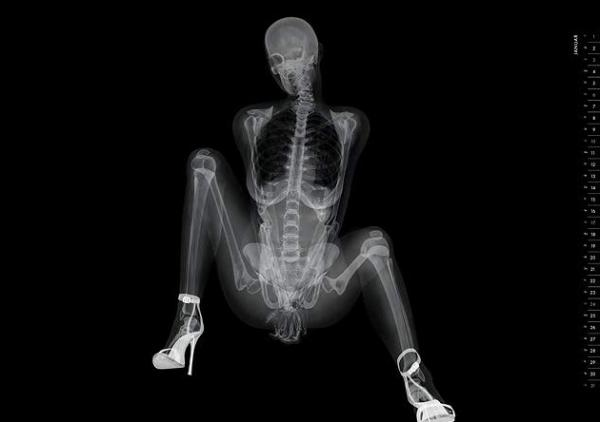
\includegraphics[width=7cm]{frontpage2}% <-this % stops a space
%  \IEEEcompsocitemizethanks{\IEEEcompsocthanksitem M. Shell is with the Department
%    of Electrical and Computer Engineering, Georgia Institute of Technology, Atlanta,
%    GA, 30332.\protect\\
%    % note need leading \protect in front of \\ to get a newline within \thanks as
%    % \\ is fragile and will error, could use \hfil\break instead.
%    E-mail: see http://www.michaelshell.org/contact.html
%    \IEEEcompsocthanksitem J. Doe and J. Doe are with Anonymous University.}% <-this % stops a space
%  \thanks{Manuscript received April 19, 2005; revised January 11, 2007.}
}

% note the % following the last \IEEEmembership and also \thanks - 
% these prevent an unwanted space from occurring between the last author name
% and the end of the author line. i.e., if you had this:
% 
% \author{....lastname \thanks{...} \thanks{...} }
%                     ^------------^------------^----Do not want these spaces!
%
% a space would be appended to the last name and could cause every name on that
% line to be shifted left slightly. This is one of those "LaTeX things". For
% instance, "\textbf{A} \textbf{B}" will typeset as "A B" not "AB". To get
% "AB" then you have to do: "\textbf{A}\textbf{B}"
% \thanks is no different in this regard, so shield the last } of each \thanks
% that ends a line with a % and do not let a space in before the next \thanks.
% Spaces after \IEEEmembership other than the last one are OK (and needed) as
% you are supposed to have spaces between the names. For what it is worth,
% this is a minor point as most people would not even notice if the said evil
% space somehow managed to creep in.



% The paper headers
\markboth{MRI: Asger Dam Hoedt - 20051770, Thomas Salomon - 2005xxxx, Peter Kristensen - 2005yyyy, 2010}%
         {MRI: Medical Resonance Imaging Simulation using the GPGPU}

% \markboth{Journal of \LaTeX\ Class Files,~Vol.~6, No.~1, January~2007}%
% {Shell \MakeLowercase{\textit{et al.}}: Bare Demo of IEEEtran.cls for Computer Society Journals}

% The only time the second header will appear is for the odd numbered pages
% after the title page when using the twoside option.
% 
% *** Note that you probably will NOT want to include the author's ***
% *** name in the headers of peer review papers.                   ***
% You can use \ifCLASSOPTIONpeerreview for conditional compilation here if
% you desire.



% The publisher's ID mark at the bottom of the page is less important with
% Computer Society journal papers as those publications place the marks
% outside of the main text columns and, therefore, unlike regular IEEE
% journals, the available text space is not reduced by their presence.
% If you want to put a publisher's ID mark on the page you can do it like
% this:
%\IEEEpubid{0000--0000/00\$00.00~\copyright~2007 IEEE}
% or like this to get the Computer Society new two part style.
%\IEEEpubid{\makebox[\columnwidth]{\hfill 0000--0000/00/\$00.00~\copyright~2007 IEEE}%
%\hspace{\columnsep}\makebox[\columnwidth]{Published by the IEEE Computer Society\hfill}}
% Remember, if you use this you must call \IEEEpubidadjcol in the second
% column for its text to clear the IEEEpubid mark (Computer Society jorunal
% papers don't need this extra clearance.)

\IEEEcompsoctitleabstractindextext{%
\begin{abstract}
  %% Isbrief:200-300words. 
%% • Summarizes your work:
%% – What problem does this paper solve?
%% – Why is this problem important for medical image computing (the context and motivation)? 
%% – How does your method work? 
%% – How does it differ from previous work? 
%% – How much better than previous work is it?
%% • There are usually no references in the abstract
%% • The abstract should be readable and understandable by non-experts

%Paralleliser gøjlet for øget hastighed. (lær at gøre det)
%Dose beregning er langsomt og ikke interaktivt endnu, parallelisering
%kan afhjælpe dette.
%Tager udgangspunkt i superposition/convolution, hvor radiological
%depth bliver beregnet vha fast raytracing.
%Gør det ikke. Men måske mere dybdegående forklaring af vores
%algoritme. (Fabs udenfor loop I hope)

In this report we present the basic principles of the physics behind
magnetic resonance imaging (MRI). Based on these we present our work
on a parallel CUDA-based implementation of an MRI-simulator. The main
kernel of the simulator is based on a discrete time-step solution to
the Bloch equations. The simulator is still at a very early stage of
development and as such does not produce correct final results. It
does however handle the effects of simple RF signals together with the
effect of phase and frequency gradients. Furthermore it samples and
visualizes the resulting signal.

%%% Local Variables: 
%%% mode: latex
%%% TeX-master: "report.tex"
%%% TeX-PDF-mode: t
%%% End: 

\end{abstract}

% Note that keywords are not normally used for peerreview papers.
\begin{IEEEkeywords}
MRI, Simulation, GPU.
\end{IEEEkeywords}}


% make the title area
\maketitle


% To allow for easy dual compilation without having to reenter the
% abstract/keywords data, the \IEEEcompsoctitleabstractindextext text will
% not be used in maketitle, but will appear (i.e., to be "transported")
% here as \IEEEdisplaynotcompsoctitleabstractindextext when compsoc mode
% is not selected <OR> if conference mode is selected - because compsoc
% conference papers position the abstract like regular (non-compsoc)
% papers do!
\IEEEdisplaynotcompsoctitleabstractindextext
% \IEEEdisplaynotcompsoctitleabstractindextext has no effect when using
% compsoc under a non-conference mode.


% For peer review papers, you can put extra information on the cover
% page as needed:
% \ifCLASSOPTIONpeerreview
% \begin{center} \bfseries EDICS Category: 3-BBND \end{center}
% \fi
%
% For peerreview papers, this IEEEtran command inserts a page break and
% creates the second title. It will be ignored for other modes.
\IEEEpeerreviewmaketitle



% An example of a floating figure using the graphicx package.
% Note that \label must occur AFTER (or within) \caption.
% For figures, \caption should occur after the \includegraphics.
% Note that IEEEtran v1.7 and later has special internal code that
% is designed to preserve the operation of \label within \caption
% even when the captionsoff option is in effect. However, because
% of issues like this, it may be the safest practice to put all your
% \label just after \caption rather than within \caption{}.
%
% Reminder: the "draftcls" or "draftclsnofoot", not "draft", class
% option should be used if it is desired that the figures are to be
% displayed while in draft mode.
%
%\begin{figure}[!t]
%\centering
%\includegraphics[width=2.5in]{myfigure}
% where an .eps filename suffix will be assumed under latex, 
% and a .pdf suffix will be assumed for pdflatex; or what has been declared
% via \DeclareGraphicsExtensions.
%\caption{Simulation Results}
%\label{fig_sim}
%\end{figure}

% Note that IEEE typically puts floats only at the top, even when this
% results in a large percentage of a column being occupied by floats.
% However, the Computer Society has been known to put floats at the bottom.


% An example of a double column floating figure using two subfigures.
% (The subfig.sty package must be loaded for this to work.)
% The subfigure \label commands are set within each subfloat command, the
% \label for the overall figure must come after \caption.
% \hfil must be used as a separator to get equal spacing.
% The subfigure.sty package works much the same way, except \subfigure is
% used instead of \subfloat.
%
%\begin{figure*}[!t]
%\centerline{\subfloat[Case I]\includegraphics[width=2.5in]{subfigcase1}%
%\label{fig_first_case}}
%\hfil
%\subfloat[Case II]{\includegraphics[width=2.5in]{subfigcase2}%
%\label{fig_second_case}}}
%\caption{Simulation results}
%\label{fig_sim}
%\end{figure*}
%
% Note that often IEEE papers with subfigures do not employ subfigure
% captions (using the optional argument to \subfloat), but instead will
% reference/describe all of them (a), (b), etc., within the main caption.


% An example of a floating table. Note that, for IEEE style tables, the 
% \caption command should come BEFORE the table. Table text will default to
% \footnotesize as IEEE normally uses this smaller font for tables.
% The \label must come after \caption as always.
%
%\begin{table}[!t]
%% increase table row spacing, adjust to taste
%\renewcommand{\arraystretch}{1.3}
% if using array.sty, it might be a good idea to tweak the value of
% \extrarowheight as needed to properly center the text within the cells
%\caption{An Example of a Table}
%\label{table_example}
%\centering
%% Some packages, such as MDW tools, offer better commands for making tables
%% than the plain LaTeX2e tabular which is used here.
%\begin{tabular}{|c||c|}
%\hline
%One & Two\\
%\hline
%Three & Four\\
%\hline
%\end{tabular}
%\end{table}


% Note that IEEE does not put floats in the very first column - or typically
% anywhere on the first page for that matter. Also, in-text middle ("here")
% positioning is not used. Most IEEE journals use top floats exclusively.
% However, Computer Society journals sometimes do use bottom floats - bear
% this in mind when choosing appropriate optional arguments for the
% figure/table environments.
% Note that, LaTeX2e, unlike IEEE journals, places footnotes above bottom
% floats. This can be corrected via the \fnbelowfloat command of the
% stfloats package.

%% • The introduction must be dynamite. 
%% – The reader forms an oppinion of the work right from the start... 
%% • The introduction is an extension of the abstract. 
%% • Should be easy to read and understand 
%% • Should make it easy for anyone to tell
%% – What your paper is about 
%%   – What problem it solves
%%   – Why the problem and solution is interesting and relevant (motivation and context). Is it a long- outstanding problem?
%%   – What is new in your paper and how (much) does it improve on the strongest alternatives/previous work (include a few of the most relevant references here).

%% • Start the introduction with the motivation. Think in large contexts and don’t be afraid to be a poet.
%% • All implications, contributions and keypoints of your work must be included here.
%% • Make it very clear how your work will impact the future of medical image computing (will people use it?).
%% • If your work is pioneering, s-p-e-l-l i-t o-u-t.
%% • Briefly make it clear how you evaluate your method in the Results section.
%% • Make sure to explain where your method applies and where it does not apply (limitations).


\section{Introduction}

% MRI, the magnetic fields, imaging

\IEEEPARstart{M}{edical} resonance imaging, MRI, is a technique used
mostly in clinical imaging to produce 3D images of patients. The
technique relies on several magnetic fields to control and measure the
spin property of atoms in the human body. Measuring every single atom
is an infeasable task and the atoms are therefore grouped into
discrete spin packets, whose net magnetization vector is a
representation of the collective spin of all atoms in the spin
packet. This net magnetization is then measured through an electric
signal it induces in the surrounding coils, postprocessed and fourier
transformed from a k-space image and back into image space.

% Focus

In this report we will focus on the basic physics of MRI and use it to
simulate the process of image acquisition. To keep the simulation
simple our program will not simulate the positioning of the net
magnetization in preparation for the signal acquisition. Here we will
instead assume that the theory is correct and analytically position
the net magnetization vectors. We will then proceed with the
simulation of the signal acquisition and storing the signal in
k-space.

% Why GPGPU?

Due to both the parallel nature of the spin packets affected by the
magnetic fields and the signal acquisition being performed identically
at discrete time intervals, MRI lends itself perfectly to dataparallel
programming. For this reason our simulator will be developed in
NVIDIA's \textbf{Compute Unified Device Architecture}, CUDA, and we
will explorer how best to utilise the Graphics Programming Unit, GPU.

% TODO Reults
TODO results

%%% Local Variables:
%%% mode: latex
%%% TeX-master: t
%%% TeX-PDF-mode: t
%%% End:


%% • Assign a special section or at least paragraph to describe your
%% contributions: What is new in this paper compared to previous work.

%% • List contributions in bullets to give a better overview.

%% • Provide a structural organization and overview of your paper: What
%% can the reader expect to read in the sections to come.

%% • Likewise start each section by clarifying what you will be
%% presenting in that section. Refer back to the overview and at the end
%% of the section, chain this section to the next section.

\section{Outline}

The structure of the article is as follows:

..

Finally we will conclude our work and present future work and
usecases.


%% S/C 

Jacques et al.\cite{sc} har tidligere vist at der kan opnås en massiv
ydelsesforbedring ved at parallelisere superposition/convolution og
lade grafikkortet om de hårde beregninger, så som raytracing til
bestemmelse af radiological depth.

% Siddon and fast raytracing

Til raytracing bliver der altid taget udgangspunkt i Siddon's linear
time raytracing algoritme fra 1985\cite{siddon}. Denne algoritme brød
med tidligere algoritmer, der alle opfattede CT data som en række
individuelle voxels, og i stedet anskuer den dataen som tre ortogonale
sæt af parallelle planer med samme afstand mellem sig.

Fox et al.\cite{fastraytracing} identificerede i 2005 problemet med at
beregne alle texture indices for alle stykker af strålen og viste
hvordan dette kunne gøres løbende mens strålen traces. De gjorde også
rede for en naiv implementation af raytracing, inspireret af
raycasting fra rendering af 3D legemer, ville lide under read-write
konflikter og hvordan dette problem kunne løses ved at skifte
synspunkt fra strålen til de enkelte voxels.


\section{MRI}
\label{sec:MRI}

% What MRI does

Magnetic Resonance Imaging is a technique used for visualizing the
amount of hydrogen atoms present in a patient. Each voxel in the image
corrosponds to a spin packet and the intensity in the voxel is an
approximation of how many hydrogen atoms was present within that
particular spin packet. This is useful in medical imaging as different
materials such as blood, bones and brain matter will produce different
intensities and can thus be distinguised in the images.

% The B0 magnetic field

To control the direction of the hydrogen's nucleus spin several
magnetic fields are employed. The first is a static field called
$\mathbf{B}_0$ aligned along the length of the patiens body from toe
to head. In clinical imaging this is taken as the z-axis. The effect
of applying $\mathbf{B}_0$ is to align all spin packets net
magnetization vectors along the z-axis. The net magnetization vector
is then said to be at equilibrium. This does not mean that all the
individuel spins of the hydrogens nuclei are pointing upwards, but the
sum of all spindirections will produce a vector along the z-axis. The
individuel spins are also precessing about the z-axis, but while the
net magnetization is at equilibrium this precessing is not measurable.

% RF pulse

While at equilibrium the net magnetization vector doesn't produce any
signal. To induce a signal in the surrounding coils the net
magnetization will have to be flipped into the transverse plane,
ie. the xy-plane. To flip the magnetization another magnetic field,
$\mathbf{B}_1$, is used. This is called the RF field. Once the net
magnetization vector has been rotated into the transverse plane, the
RF field is turned off. The magnetic spin is again only affected by
$\mathbf{B}_0$ and will therefore return to equilibrium. Because the
net magnetization vector is still precessing about the z-axis, the
spin will then induce a signal in the surrounding coils, which can be
used to create the image.

% Distinquishing signals with Slice selection, frequency encoding and
% pulse encoding

If all net magnetizations are flipped at the same time it will be
impossible to distinguish their signal and the resulting image will
consist of one gray voxel. A gradient field consisting of several
smaller magnetic fields are therefore used to distinguish the
individuel spin packets.

The first is a slice selection gradient field, $\mathbf{B}_{G_s}$,
which when applied will make only one slice react to the
$\mathbf{B}_1$ field, and therefore the coil will only receive signals
from spin packets in that slice.

The second gradient field, $\mathbf{B}_{G_\phi}$, phase shifts the net
magnetizations transverse spin. What this means is that the transverse
spin of the net magnetizations are brought out of phase with the other
netmagnetizations in the slice, thus giving them a uniquely detectable
rotation. And the third gradient field, $\mathbf{B}_{G_f}$, is a
linear magnetic field gradient. The effect of $\mathbf{B}_{G_f}$ is to
encode the frequency at which the net magnetization precesses in the
transverse plane.

These last 2 gradients will make it possible for a fourier transform
to 'recoqnize' the individuel spin packets and recreate the original
image.

%%% Local Variables: 
%%% mode: latex
%%% TeX-master: "report.tex"
%%% TeX-PDF-mode: t
%%% End: 


\section{Magnetic Fields}

% Magnetic fields

We are interested in modeling the behaviour of the net magnetization,
$\textbf{M}$, of spin packets under the influence of one or more
magnetic fields. This is a function dependent on the time, $t$, and
position, $\textbf{p}$, within the sample. The functions describing
each coordinate component of $\textbf{M}$ are $M_x$, $M_y$ and
$M_z$. Thus our net magnetization is given by

\begin{displaymath}
  \textbf{M}(t, \textbf{p}) = \langle M_x(t, \textbf{p}), M_y(t, \textbf{p}), M_z(t, \textbf{p}) \rangle
\end{displaymath}

As stated previously, when only the static magnetic field
$\mathbf{B}_0 = \langle 0, 0, B_0 \rangle$ is active, $\textbf{M}$
will lie at equilibrium along the z-axis. Thus $\textbf{M} = \langle
0, 0, M_{eq} \rangle$, where $M_{eq}$ is the magnitude of $\textbf{M}$.

The gyromagnetic ratio, $\gamma$, of a particle is the ratio of it's
magnetic dipole moment to it's angular momentum. This means that
$\gamma$ can tell us how fast the net magnetization will precess
around the magnetic field applied to it. 

\begin{displaymath}
  \omega = \gamma \| \mathbf{B} \|
\end{displaymath}

The gyromagnetic ratio for hydrogen atoms is $42.58 \cdot 10^6 Hz / T$
(hertz pr. tesla).

With this we can now formulate the bloch equations that descripe the
net magnetizations rate of change over time with respect to the sum of
magnetic fields, $\mathbf{B}$.

% Bloch equations
\begin{displaymath}
  \frac{d\mathbf{M}}{dt} = \gamma \mathbf{M} \times \mathbf{B} -
  \frac{\langle M_x, M_y, 0 \rangle}{T_2} - \frac{\langle 0, 0, M_z -
    M_{eq} \rangle}{T_1}
\end{displaymath}

$T_1$ and $T_2$ are relaxation times for the spins. $T_1$ is the
\textit{spin-lattice} relaxation time and describe how fast the net
magnetization will return to equilibrium. $T_2$ is the
\textit{spin-spin} relaxation time and reflects how fast the magnitude
of the net magnetizations transverse components goes to 0. $T_2$ will
always be smaller or equal to $T_1$.

% @TODO figures of relaxation times

% Magnetic fields

As explained earlier $\mathbf{B}$ is the sum of three magnetic fields;
the static field $\mathbf{B}_0$, the RF field $\mathbf{B}_1$ and the
gradient field $\mathbf{B}_G$.

\begin{displaymath}
  \mathbf{B} = \mathbf{B}_0 + \mathbf{B}_1 + \mathbf{B}_G
\end{displaymath}

The static field, as written earlier, is simply $\mathbf{B}_0 =
\langle 0, 0, B_0 \rangle$, which is a magnetic field lying along the
z-axis. $\mathbf{B}_0$ causes the spin of the nuclei to precess about
the z-axis at frequency $\gamma B_0 = \omega_0$.

The RF magnetic field, or RF pulse, $\mathbf{B}_1$ is more complex. It
has to rotate the net magnetization 90 degrees into the transverse
plane, while the aggregate magnetic moment is precessing about the
$\mathbf{B}_0$ field. In order to do that $\mathbf{B}_1$ is itself
rotating about $\mathbf{B}_0$ at frequence $\omega_0$.

\begin{displaymath}
  \mathbf{B}_1 = \langle B_1 cos(\omega_0 t), B_1 sin(\omega_0 t), 0\rangle
\end{displaymath}

The $\mathbf{B}_1$ field does not simply rotate the net magnetization
instantly. Instead it needs to be active at a specific time interval
$\tau_{90\degree}$. The time interval can be calculated using

\begin{displaymath}
  \tau_{90\degree} = \frac{1 / 4}{\gamma * \|\mathbf{B}_1\|}
\end{displaymath}

\subsection{Magnetic field gradients}

\begin{figure}
  \centering
  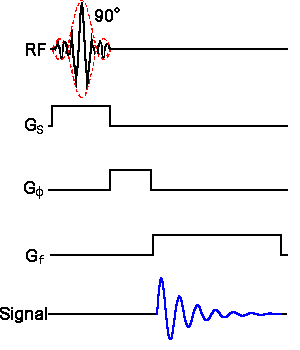
\includegraphics[width=5cm]{gradientSequence}
  \caption{A timing diagram of the application of gradients with
    respect to the RF pulse and signal acquisition.}
  \label{fig:gradientSequence}
\end{figure}

Recall from earlier that if all net magnetizations are spinning in the
same phase and at the same frequency, they are indistinguishable to
the fourier transform and thus produces on image with only one
voxel. We will now in more detail present the gradient fields that
help distinguish the individual spin packets.

We have previously included the gradient fields in our equations as
one variable, $\mathbf{B}_G$. This is purely done to simplify the
equations. In practice one must remember that the gradient field
actually consists of the 3 seperat gradient fields described in
\refsec{sec:MRI}.

\begin{displaymath}
  \mathbf{B}_G = \mathbf{B}_{G_s} + \mathbf{B}_{G_\phi} + \mathbf{B}_{G_f}
\end{displaymath}

As can be seen on \reffig{fig:gradientSequence} the individual
gradients are never active at the same time.

The strenght of all the gradient fields applied are linearly
increasing along a given normal, $\mathbf{G}$, and all gradient fields
have the same direction as $\mathbf{B}_0$. The generel equation for a
gradient field thus becomes.

\begin{displaymath}
  \mathbf{B}_G(\mathbf{p}) = \langle 0, 0, \mathbf{G} \cdot \mathbf{p} \rangle
\end{displaymath}


The first gradient field that is applied is the slice selection
gradient, which is active together with the RF field. As previously
described $\mathbf{B}_{G_s}$ is responsable for ensuring that only a
slice through the patient is affected by the RF pulse and thus that
only this slice will produce a signal. In the theory behind MRI this
slice is placed in the xy-plane with a normal $\langle 0, 0, G_s
\rangle$ and the gradient field is therefore

\begin{displaymath}
  \mathbf{B}_{G_s}(\mathbf{p}) = \langle 0, 0, G_s p_z \rangle
\end{displaymath}


% The y-axis is the phase encode direction and is phase encoded with a
% phase gradient.

The next gradient field applied is phase encoding gradient,
$\mathbf{B}_{G_\phi}$. This is applied to distinguish rotations along
the y-axis and therefore has the form

\begin{displaymath}
  \mathbf{B}_{G_\phi}(\mathbf{p}) = \langle 0, 0, G_\phi p_y \rangle
\end{displaymath}

\begin{figure}
  \centering
  \subfigure[In phase.]{
    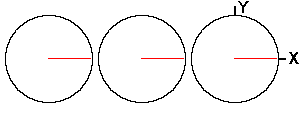
\includegraphics[width=5cm]{inPhase}
  }
  \subfigure[Out of phase.]{
    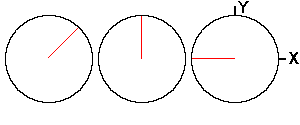
\includegraphics[width=5cm]{outOfPhase}
  }
  \caption{Figures of in-phase and phase shifted net
    magnetizations. Here the phase shift is along the x-axis.}
  \label{fig:phaseShift}
\end{figure}

With the phase encoding gradient active, each net magnetization vector
along the y-axis will precess at it's own unique larmor frequency. 

\begin{displaymath}
  \omega_\phi(\mathbf{p}) = \gamma (B_0 + B_{G_\phi} \cdot p_y)
\end{displaymath}

It therefore follows that when the phase encode gradient is turned
off, all the net magnetization vectors will return to precessing at
the same larmor frequency, $\omega_0$, but out of phase with each
other, as can be seen on \reffig{fig:phaseShift}. In
\refsec{sec:imaging} we shall see how this enables the fourier
transform to distinguish spin packets along the y-axis.

To enable the fourier transform to reconstuct the intensity of a given
spin packet, we need the phase encoding oscilate. This is achieved by
letting the strength of the phase gradient, $B_{G_\phi}$, start at
$G_{\phi_{max}}$ for the first slice excitation and then linearly drop to
$-G_{\phi_{max}}$ in the last excitation.

%TODO phase time and calculating strength



% Constant gradient field along the x axis. The strength of the
% gradient field increases along the x-axis and never changes over the
% course of the signal acquisition.

The final gradient field is the frequency encoding gradient that
encodes the signal along the x-axis.

\begin{displaymath}
  \mathbf{B}_{G_f}(\mathbf{p}) = \langle 0, 0, G_f p_x \rangle
\end{displaymath}

The frequency encoding gradient is turned on while aquirering the
data, to give all net magnetizations along the x-axis their own larmor
frequency.

\begin{displaymath}
  \omega_f(\mathbf{p}) = \gamma (B_0 + B_{G_f} \cdot p_x)
\end{displaymath}

TODO time and strength?

While we here have placed all gradient fields along a specific axis in
our coordinate system, one should remember that we are free to place
the coordinate system in any way we like and thus the theory
generalizes to gradients in any direction, which is useful for oblique
image acquisition.






%%% Local Variables:
%%% mode: latex
%%% TeX-master: t
%%% TeX-PDF-mode: t
%%% End:


\section{Imaging}
\label{sec:imaging}

% http://en.wikipedia.org/wiki/Free_induction_decay
% In Fourier Transform NMR, a free induction decay (FID) is the
% observable NMR signal generated by non-equilibrium nuclear spin
% magnetisation precessing about the magnetic field (conventionally
% along z). 

The observable signal used for imaging is a free induction decay, FID,
generated by non-equilibrium nuclear spin magnetization precessing
about the magnetic field

% B1 magnetic field

%% To distinguish slices in the body, a gradient field, $B_{G_s}$, is applied
%% along the z-axis. The gradient field varies along the z-axis, with
%% only a 0 Tesla effect in the slice that should be excited. Since the
%% frequency of the photons that can excite a spin is linearly
%% proportional to the strength of the magnetic field on that spin, it
%% follows that the photons of frequency $\omega_0 = \gamma B_0$ will
%% only affect spin packets unaffected by the gradient $B_{G_s}$. Applying
%% $B_{G_s}$ for the duration of the RF pulse ensures that only spin packets
%% in the slice is excited and will produce a signal during the signal
%% acquisition phase.



By Faraday's law of induction the signal generated by a single spin
packet is \cite{feeman}

\begin{displaymath}
  M^*(t, \mathbf{p}) = M_x(t, \mathbf{p}) + i \cdot M_y(t, \mathbf{p})
\end{displaymath}

The complete signal from the excited slice is then

\begin{displaymath}
    M^*(t) = \sum^{(X, Y)}_{(x',y')} (M_x(t, \mathbf{p_{(x',y')}}) + i \cdot M_y(t, \mathbf{p_{(x',y')}}))
\end{displaymath}

which is sampled in intervals of $t$ for the duration $\tau$.


The number of samples taken during each excitation is directly
proportional to the image resolution along the x-axis. The resolution
along the y-axis is given by how many times a slice is excited and
sampled.


\subsection{K-space}

The signal acquired is stored in K-space. Each specific excited slice
in the patient corrosponds to a two dimensional K-space image with
complex entries. A row in the image along the x-axis, the frequency
encoding direction, hold signals sampled over time $\tau$ at intervals
$t$ after one application of the RF pulse. All the lines along the
y-axis, the phase encoding direction, represent samples with different
phase encodings. An example of a K-space image can be seen in
\reffig{fig:kSpace}, where two net mangnetizations have produced a
signal.

With the information in K-space it is possible to restore the original
hydrogen intensities from the sampled FID signal. Fourier transforming
the image in \reffig{fig:kSpace} in its frequency encoding direction,
yields the frequency domain information seen in
\reffig{fig:frequencyDomain}. Fourier transforming this in the phase
encoding direction will give us the hydrogen intensities of the spin
packets, as can be seen in \reffig{fig:phaseDomain}. Here we can also
see why the phase encoding gradient varies for each excitation, as
that gives the oscilation along the phase encoding direction.


% Perform 2D fourier transform of the data in k-space, cuda does this
% with Sangilds wrapper

\begin{figure}
  \centering
  \subfigure[K-space]{
    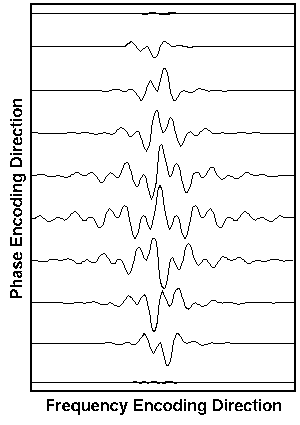
\includegraphics[width=4.5cm]{kSpace}
    \label{fig:kSpace}
  }
  \subfigure[Frequency domain information extracted by performing a
    Fourier transform along the x-axis.]{
    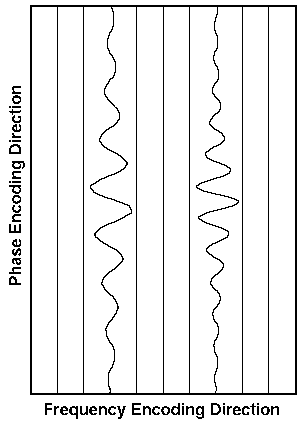
\includegraphics[width=4.5cm]{frequencyDomain}
    \label{fig:frequencyDomain}
  }
  \subfigure[Frequency and phase domain information extracted by performing a
    2D Fourier transform along the x- and y-axis.]{
    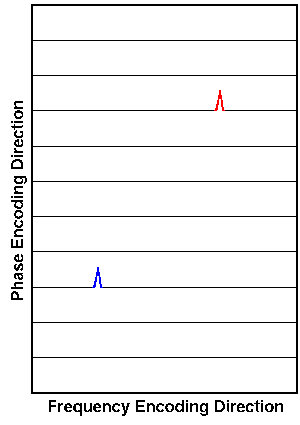
\includegraphics[width=4.5cm]{phaseDomain}
    \label{fig:phaseDomain}
  }
  \caption{The effect from fourier transforming a K-space image.}
  \label{fig:kSpaceTransformations}
\end{figure}

The one dimensional fourier transform is given by 

\begin{displaymath}
  \begin{array}{rl}
    f(\omega) &= \int^\infty_{-\infty}f(t)e^{-i \omega t} dt \\
    &= \int^\infty_{-\infty}f(t)(\cos(\omega t) - i \sin(\omega t)) dt \\
    &\approx \sum^\infty_{-\infty}f(t)(\cos(\omega t) - i \sin(\omega t))
  \end{array}
\end{displaymath}

% The signal strength is the length of the complex number from the
% fourier transform, not just the real component.

Since the fourier transform is both applied to and returns complex
numbers, the hydrogen intensity produced by a two dimensional
transform is also a complex number, $h'$. Converting this to the
final intensity, $h$, is done by taking the modulus of the complex
intensity.

\begin{displaymath}
  h = \|h'\| = \|h'_{real} + i h'_{imaginary}\| = \sqrt{h_{real}^{'2} + i h_{imaginary}^{'2}}
\end{displaymath}


%%% Local Variables: 
%%% mode: latex
%%% TeX-master: "report.tex"
%%% TeX-PDF-mode: t
%%% End: 


\section{Implementation}

% model the B0 and BGf fields

% Assume slice selection and possibly phase gradient

In our simulation we assume that the correct slice has been selected
and excited, so we only work with a 2 dimensional image and the net
magnetization vectors have been rotated into the transversal
plane. This allows us to focus on the image acquisition phase.

% Bloch equations with the gradient and B0, which is what we're
% solving

With only the static magnetic field $\mathbf{B}_0$ and
$\mathbf{B}_{G_f} = \langle 0, 0, p_x * B_{G_f} \rangle$ active, the
block equations simply to

\begin{displaymath}
  \begin{array}{l}
    \frac{dM_x}{dt} = \gamma (B_0 + p_x * B_{G_f}) M_y - \frac{M_x}{T_2} \\
    \frac{dM_y}{dt} = - \gamma (B_0 + p_x * B_{G_f}) M_x - \frac{M_y}{T_2} \\
    \frac{dM_z}{dt} = - \frac{M_z - M_{eq}}{T_1}
  \end{array}
\end{displaymath}

which have the analytical solution 

\begin{displaymath}
  \begin{array}{l}
    M_x(t) = e^{-t/T_2}(M_x(0) cos(w_0 t + w_f t) - M_y(0) sin (w_0 t + w_f t)) \\
    M_y(t) = e^{-t/T_2}(M_x(0) sin(w_0 t + w_f t) + M_y(0) cos (w_0 t + w_f t)) \\
    M_z(t) = M_z(0) e^{t/T_1} + M_eq(1 - e^{-1/T_1})
  \end{array}
\end{displaymath}

% One kernel for Calculating several/all timesteps and store them in
% an array. (one thread pr voxel in the original image)

% Then have one kernel sum up the signal and write it in out k-space
% image.

% A last kernel will transform the image back to image space. Use
% Sangilds fft wrapper.

% If this image looks like crap then we don't care! Some mumbo jumbo
% about where it might have gone wrong, possible some images showing
% the net magnetization (with color interpretation) and then that's
% all she wrote.

%%% Local Variables:
%%% mode: latex
%%% TeX-master: t
%%% TeX-PDF-mode: t
%%% End:



\section{Conclusion}

%%% Local Variables:
%%% mode: latex
%%% TeX-master: t
%%% TeX-PDF-mode: t
%%% End:


\section{Future Work}

%%% Local Variables: 
%%% mode: latex
%%% TeX-master: "report.tex"
%%% TeX-PDF-mode: t
%%% End: 



% use section* for acknowledgement
%\ifCLASSOPTIONcompsoc
  % The Computer Society usually uses the plural form
%  \section*{Acknowledgments}
%\else
  % regular IEEE prefers the singular form
%  \section*{Acknowledgment}
%\fi


%The authors would like to thank...


% Can use something like this to put references on a page
% by themselves when using endfloat and the captionsoff option.
\ifCLASSOPTIONcaptionsoff
  \newpage
\fi



% trigger a \newpage just before the given reference
% number - used to balance the columns on the last page
% adjust value as needed - may need to be readjusted if
% the document is modified later
%\IEEEtriggeratref{8}
% The "triggered" command can be changed if desired:
%\IEEEtriggercmd{\enlargethispage{-5in}}

% references section

% can use a bibliography generated by BibTeX as a .bbl file
% BibTeX documentation can be easily obtained at:
% http://www.ctan.org/tex-archive/biblio/bibtex/contrib/doc/
% The IEEEtran BibTeX style support page is at:
% http://www.michaelshell.org/tex/ieeetran/bibtex/
%\bibliographystyle{IEEEtran}
% argument is your BibTeX string definitions and bibliography database(s)
%\bibliography{IEEEabrv,../bib/paper}
%
% <OR> manually copy in the resultant .bbl file
% set second argument of \begin to the number of references
% (used to reserve space for the reference number labels box)
\begin{thebibliography}{4}

%\bibitem{IEEEhowto:kopka}
%H.~Kopka and P.~W. Daly, \emph{A Guide to \LaTeX}, 3rd~ed.\hskip 1em plus
%  0.5em minus 0.4em\relax Harlow, England: Addison-Wesley, 1999.

\bibitem{siddon}
R. L. Siddon, \emph{Fast calculation of the exact radiological path for a three-
dimensional CT array}, Med. Phys. (1985) 12(2), 252–258.

\bibitem{sc} 
R. Jacques, et al., \emph{Towards real-time radiation therapy: GPU
  accelerated superposition/convolution}, Comput.  Methods Programs
Biomed. (2009), doi:10.1016/j.cmpb.2009.07.004

\bibitem{fastraytracing} 
C. Fox, H. E. Romeijn and J. F. Dempsey, \emph{Fast voxel and polygon
ray-tracing algorithms in intensity modulated radiation therapy
treatment planning}, Med. Phys. (2006) 33 1364–71

\bibitem{convolution}
T.~R.~Mackie, J.~W.~Scrimger and J.~J.~Battista, \emph{A convolution method
of calculating dose for 150MV x rays}, Med. Phys. (1985) 12(2):188-196

\end{thebibliography}

% biography section
% 
% If you have an EPS/PDF photo (graphicx package needed) extra braces are
% needed around the contents of the optional argument to biography to prevent
% the LaTeX parser from getting confused when it sees the complicated
% \includegraphics command within an optional argument. (You could create
% your own custom macro containing the \includegraphics command to make things
% simpler here.)
%\begin{biography}[{\includegraphics[width=1in,height=1.25in,clip,keepaspectratio]{mshell}}]{Michael Shell}
% or if you just want to reserve a space for a photo:

%\begin{IEEEbiographynophoto}{Asger Dam Hoedt}
%Biography text here.
%\end{IEEEbiographynophoto}

% You can push biographies down or up by placing
% a \vfill before or after them. The appropriate
% use of \vfill depends on what kind of text is
% on the last page and whether or not the columns
% are being equalized.

%\vfill

% Can be used to pull up biographies so that the bottom of the last one
% is flush with the other column.
%\enlargethispage{-5in}


% if have a single appendix:
%\appendix[Proof of the Zonklar Equations]
% or
%\appendix  % for no appendix heading
% do not use \section anymore after \appendix, only \section*
% is possibly needed

% use appendices with more than one appendix
% then use \section to start each appendix
% you must declare a \section before using any
% \subsection or using \label (\appendices by itself
% starts a section numbered zero.)
%

\appendices
\section{Running the program.}

Instuktioner til at installere programmet kan findes på
http://www.openengine.dk/trac/wiki/Projects/DeathRay. 

Programmet er allerede installeret på Christian Christoffersen's
computer, så for at slippe for alt bøvlet med at installere
dependencies, kan det anbefales at køre det der.


\onecolumn


\section{CUDA kernels}

%\lstinputlisting[language=C]{Superposition.cu}



% that's all folks
\end{document}


